\chapter{Analysis types and time integration}
\label{ch:analyses}

\code{RunSimulation} selects the analysis with \code{settings.analysis_type} and
calls one of four functions in \code{subroutines/AnalysisType}. Before that it
sets up the $3\times3$ material matrix of every material with
\code{MaterialMatrices} (2 constants: isotropic \code{HookeMatrix3d}; 9 constants:
orthotropic), reduced to plane stress or plane strain, and the Rayleigh parameters
(\code{RayleighDamping}). All four functions assemble through
\code{AssembleSystem} (a wrapper of \code{AssemblyFEM} for the \code{model}
struct) and return a struct \code{results}; \code{help}~\code{StaticAnalysis} etc.\ list
its fields.

\section{Static analysis (\texttt{StaticAnalysis})}

\begin{enumerate}
  \item Assemble $\matr K$ (\code{flag_comp = 0}).
  \item Find the homogeneous Dirichlet DOFs.
  \item Assemble the loads (\code{NeumannBCs}).
  \item Apply the prescribed displacements (\code{DirichletBCs_nonhomogeneous}).
  \item Solve $\matr K_\mathrm{aa}\vect u_\mathrm{a} = \vect F_\mathrm{a}$ with \texttt{\textbackslash}
    (sparse LU, since $\matr K$ is unsymmetric).
\end{enumerate}
\code{RunSimulation} then saves the results (\code{SaveResults}) and plots them
(\code{PlotResults} $\to$ \code{Contour_plot}).

\section{Dynamic analysis (\texttt{DynamicAnalysis})}
\label{sec:dynamic}

\begin{enumerate}
  \item \code{AssemblyFEM(..., 2)}: $\matr K$, $\matr M$, Rayleigh $\matr R$ and
    the stable time step \code{dte} of the central difference method.
  \item Assemble the loads, with one column per load case if \code{flag_mRHS}.
    Prescribed displacements are handled by lifting
    (\code{DirichletBCs_nonhomogeneous_dynamic}).
  \item Collect the input of the solver in a struct \code{S} (matrices, loads,
    initial conditions, DOF sets, time step candidates, signal, options) and call
    \code{Solver_Transient(S)}. It reduces everything to the active DOFs, chooses
    the method from \code{TimeIntegrationMethods} and passes it the time step
    candidates \code{dt = [dtf, dte, TimeIntegration.dtImp]}.
    \code{dtf = 0.05/f_max} gives 20 samples per period of the highest excited
    frequency (\code{FFT_Signal}); the simulation time is \code{settings.t_end},
    or the time period of the \texttt{ABAQUS} step if it is empty.
  \item By default only the nodes of interest are stored (\code{save_var = 0}).
\end{enumerate}
With \code{TimeIntegration.SolverSave = true}, \code{S} is also written to
\code{subroutines/Temp/Solver_input.mat}; \code{Solver_Transient} accepts this
file name instead of the struct, so a time integration can be repeated (e.g.\
with another method) without the preprocessing:
\begin{lstlisting}
S = load(fullfile(settings.TempFolder, 'Solver_input.mat'));
S.TimeIntegration.Method = 303;          % generalized-alpha instead
[T, U] = Solver_Transient(S);
\end{lstlisting}

\paragraph{Important.} With \code{flag_mRHS = true} (the default)
\code{Solver_Transient} ignores the method code. It runs
\code{CentralDifferenceMethod_mRHS} for codes below 300 and
\code{HHTAlphaMethod_mRHS} otherwise.

\paragraph{Time step selection inside the integrators.} Explicit schemes use
\code{dt = min(dtmax)} after scaling \code{dte} by the stability factor of the
method; implicit schemes use \code{dt = dtImp} if all three entries differ,
otherwise \code{dtf}. The step is then adjusted to \code{tsim/ceil(tsim/dt)}.
Both rules are implemented once, in \code{TimeIntegration/Common/TimeStepSize}.

\begin{xltabular}{\linewidth}{@{}P{1.4cm}P{6.0cm}L@{}}
  \caption{Time integration methods (\texttt{TimeIntegration.Method}); the
    same table is in \texttt{TimeIntegrationMethods.m}, which
    \texttt{Solver\_Transient} uses to find the routine and its extra
    arguments.}
  \label{tab:methods}\\
  \toprule
  code & routine & remarks \\
  \midrule
  \endfirsthead
  \toprule
  code & routine & remarks \\
  \midrule
  \endhead
  101, 601 & \code{CentralDifferenceMethod} & explicit, 2nd order \\
  102 & \code{NohBatheMethod} & explicit, $p = 0.54$ \\
  103 & \code{SoaresMethodExplicit} & \\
  104 & \code{MirbagheriMethod} & Noh-Bathe with the factor $\eta = 1.025$ on the
    acceleration term of the predictor (dissipation against spurious
    oscillations); first order by design \\
  105 & \code{KimMethodExplicit} & \\
  106, 107 & \code{ZhangXingMethod1}, \code{ZhangXingMethod2} & $\rho = 1$ and
    $\rho = 0$ \\
  108 & \code{ExplicitGeneralizedAlphaMethod} & $\rho_\mathrm{b} = 1$ \\
  109 & \code{AdaptiveHybridExplicitMethod} & adaptive hybrid explicit method
    \parencite{Soares2020novel}, \cref{sec:ahem} \\
  201 & \code{KimExplicit_ho} & order 3 or 4 \\
  202 & \code{KimMethod2Stage} & two-stage explicit method \\
  301 & \code{NewmarkMethod} & trapezoidal rule $\beta = 1/4$, $\gamma = 1/2$;
    also the fallback for unknown codes \\
  302 & \code{HHTAlphaMethod} & $\alpha = -0.05$ \\
  303 & \code{GeneralizedAlphaMethod} & $\rho_\infty = 0.8$ \\
  304 & \code{BatheBaigMethod} & \\
  305 & \code{b1b2_BatheMethod} & $\beta_1 = 1/3$ \\
  306 & \code{rho_BatheMethod} & $\rho_\infty = 0$ \\
  307 & \code{SoaresMethodImplicit} & \\
  308, 309 & \code{KimMethodImplicit}, \code{KimMethodImplicitCollocation} & \\
  401 & \code{KimLagrange_ho} & order 1--5 \\
  402 & \code{SoaresMethodImplicit_ho} & \\
  403 & \code{PadeMethod} $\to$ Padé-based integrators & order \code{Order} =
    2--10; $\rho_\infty$ = \code{TimeIntegration.rho} (1:
    \code{PadeTimeIntegrator}, ${}<1$: \code{PadeTimeIntegrator_ND}, or the
    \texttt{Fortran} solver if it is on the path); loads: see \cref{ch:issues} \\
  501 & \code{HPTIM_Newmark} & highly precise time integration; currently not
    functional (\cref{ch:issues}) \\
  \bottomrule
\end{xltabular}

\paragraph{Common calling convention.} All methods are called as
\begin{lstlisting}
[T, U(, V, A)] = Method(K, M, C, F, F_dt, U0, V0, NumDoF, DOFsave, ...
                        ActiveDoFs, ExciteParam, SignalType, dtmax, ...
                        tsim [, extra])
\end{lstlisting}

\begin{xltabular}{\linewidth}{@{}P{4.2cm}L@{}}
  \toprule
  argument & meaning \\
  \midrule
  \code{K}, \code{M}, \code{C} & reduced (active-DOF) matrices \\
  \code{F} & constant load (applied at $t = 0$) \\
  \code{F_dt} & time-dependent load: a vector, or a struct with the fields
    \code{.Neumann}, \code{.K}, \code{.C}, \code{.M}, multiplied by $s(t)$,
    $s(t)$, $\dot s(t)$ and $\ddot s(t)$ \\
  \code{U0}, \code{V0} & initial displacement and velocity; the initial
    acceleration follows from the equation of motion \\
  \code{NumDoF}, \code{DOFsave}, \code{ActiveDoFs} & total DOFs, stored (reduced)
    DOFs, map from reduced to global DOFs \\
  \code{dtmax} & \code{[dtf, dte, dtImp]} \\
  \code{tsim} & simulation time \\
  \code{extra} & waitbar flag (central difference), order (higher-order
    methods) or element data (method 109) \\
  \code{T}, \code{U}, \code{V}, \code{A} & time vector and histories
    \texttt{[nT+1 x numel(DOFsave)]}, expanded to all DOFs if all active DOFs are
    stored; the \code{_mRHS} variants return 3-D arrays (time $\times$ DOF
    $\times$ load case) \\
  \bottomrule
\end{xltabular}
\code{tests/unit/TimeIntegrationTest.m} verifies the accuracy and the
convergence order of the schemes on a 2-DOF oscillator.

\paragraph{Shared building blocks.} The steps that every method needs are in
\code{TimeIntegration/Common}; \code{NewmarkMethod} (implicit) and
\code{CentralDifferenceMethod} (explicit) show how they fit together, and
\cref{sec:dev-integrator} explains how to add a method.

\begin{xltabular}{\linewidth}{@{}P{6.4cm}L@{}}
  \toprule
  routine & purpose \\
  \midrule
  \code{[dt, n] = TimeStepSize(dtmax, tsim [, factor])} & time step: implicit
    rule, or explicit rule with the stability factor of the method relative to
    the central difference method \\
  \code{[K, M, C, Fdt] = PrepareSystem(K, M, C, F_dt, nActive)} & full matrices
    from triangular storage; load parts as a struct \\
  \code{[s, ds, dds] = SignalHistory(SignalType, ExciteParam, t)} & excitation
    signal and its derivatives at the times \code{t} \\
  \code{Ft = LoadAtTime(F, Fdt, s, ds, dds)} & load vector at one instant \\
  \code{a0 = InitialAcceleration(solveM, F, Fdt, K, C, u0, v0, ...)} &
    acceleration at $t = 0$ from the equation of motion \\
  \code{[U, V, A] = ExpandToAllDoFs(NumDoF, ActiveDoFs, u, v, a)} & histories
    of all DOFs if every active DOF was stored \\
  \code{pb = ProgressBar(name, n [, enabled])} & waitbar with
    \code{pb.update(i)}, \code{pb.close()} \\
  \bottomrule
\end{xltabular}

\subsection{Adaptive hybrid explicit method (109)}
\label{sec:ahem}

The implementation follows Table~1 of \textcite{Soares2020novel}.
\begin{itemize}
  \item \textbf{Elements.} Every element $e$ gets its maximum sampling frequency
    $\Omega_e = \omega_{\max,e}\,\Delta t$ from its own (unsymmetric)
    eigenproblem $\matr K_e\bm\phi = \omega^2\matr M_e\bm\phi$. Elements with
    $\Omega_e \le 2$ use the \emph{regular} formulation (stability limit 2, one
    stiffness product per step); elements with $2 < \Omega_e \le 4$ use the
    \emph{enhanced} formulation (stability limit 4, an additional correction of
    the displacements).
  \item \textbf{Time step.} $\Delta t = 2\,\Delta t_\mathrm{CDM}$, twice the
    critical time step of the central difference method (\code{dte} from
    \code{AssemblyFEM}).
  \item \textbf{Adaptive dissipation.} Numerical damping is switched on only in
    elements in which a DOF oscillates, i.e.\ where its last two increments have
    opposite signs (exact form of the oscillatory criterion, Eq.~(7) of the
    paper). The parameters $\alpha_e$ (Eq.~(8b), capped at 3) and $\beta_e$
    (Eq.~(12b)) place the bifurcation of the amplification matrix at $\Omega_e$,
    so the stability limit is not reduced (\cref{fig:ahem}).
  \item \textbf{Damping.} Rayleigh damping is supported; the damping ratio of
    Eqs.~(8b) and (12b) is computed from the mass-proportional part,
    $\zeta_e = \alpha_\mathrm{R}\,\Delta t/2$.
  \item \textbf{Requirements.} For method 109 \code{DynamicAnalysis} requests
    the element matrices from \code{AssemblyFEM} (6th output \code{ElemData}) and
    passes them to the solver (field \code{S.ElemData}). Set
    \code{flag_mRHS = false}, otherwise the method code is ignored. Use lumped
    mass matrices (\code{mass_matrix = 2}, GLL nodal quadrature): then
    $\matr E = \matr M + \tfrac12\Delta t\,\matr C$ is diagonal and no linear
    solver is needed; consistent matrices work, but every step then solves with
    $\matr E$.
\end{itemize}

\begin{figure}[htbp]
  \centering
  % Adaptive hybrid explicit method: integration parameters alpha_e (regular
% elements, Eq. 8b, capped at 3) and beta_e (enhanced elements, Eq. 12b)
% for zeta_e = 0 as functions of the element sampling frequency Omega_e
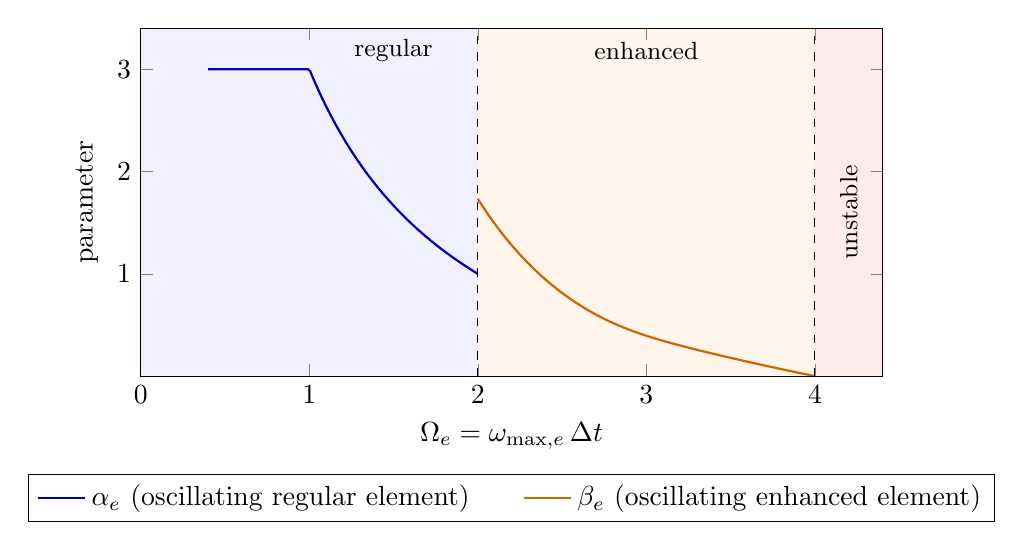
\begin{tikzpicture}
  \begin{axis}[
      width=11cm, height=6cm,
      xmin=0, xmax=4.4, ymin=0, ymax=3.4,
      xlabel={$\Omega_e=\omega_{\max,e}\,\Delta t$},
      ylabel={parameter},
      xtick={0,1,2,3,4}, ytick={1,2,3},
      legend style={at={(0.5,-0.28)}, anchor=north, legend columns=2,
                    /tikz/every even column/.append style={column sep=6mm}},
      legend cell align=left,
      every axis plot/.append style={thick},
      axis on top]
    % regions
    \fill[blue!6] (axis cs:0,0) rectangle (axis cs:2,3.4);
    \fill[orange!8] (axis cs:2,0) rectangle (axis cs:4,3.4);
    \fill[red!8] (axis cs:4,0) rectangle (axis cs:4.4,3.4);
    \node[font=\small] at (axis cs:1.5,3.18) {regular};
    \node[font=\small] at (axis cs:3,3.18) {enhanced};
    \node[font=\small, rotate=90] at (axis cs:4.2,1.6) {unstable};
    % alpha_e = min(3, 4/Omega - 1)
    \addplot[blue!70!black, domain=0.4:2, samples=120]
      {min(3, 4/x - 1)};
    \addlegendentry{$\alpha_e$ (oscillating regular element)}
    % beta_e
    \addplot[orange!80!black, domain=2.0001:4, samples=120]
      {(16 - (x^2-8)^2 + 4*sqrt(16 + 2*(x^2-8)^2))/x^4};
    \addlegendentry{$\beta_e$ (oscillating enhanced element)}
    \draw[dashed] (axis cs:2,0) -- (axis cs:2,3.4);
    \draw[dashed] (axis cs:4,0) -- (axis cs:4,3.4);
  \end{axis}
\end{tikzpicture}

  \caption{Integration parameters of the adaptive hybrid explicit method for
    $\zeta_e = 0$: $\alpha_e$ for oscillating regular elements (Eq.~(8b),
    capped at 3) and $\beta_e$ for oscillating enhanced elements (Eq.~(12b)).}
  \label{fig:ahem}
\end{figure}

\code{tests/integration/AdaptiveHybridExplicitTest.m} checks second-order
convergence, damping, and stable, accurate results at twice the
central-difference limit, where the central difference method diverges.

\section{Excitation signals}
\label{sec:signals}

The function \code{ExcitationSignal} (arguments \code{SignalType},
\code{ExciteParam}, \code{t}) returns the signal as a row vector,
\code{ExcitationSignalDerivative} (additional argument \code{order}) its
derivatives.

\begin{xltabular}{\linewidth}{@{}P{1.9cm}LP{5.0cm}@{}}
  \toprule
  \code{SignalType} & signal & \code{ExciteParam} \\
  \midrule
  0 & none & \code{tE} \\
  1 & sine burst with Hann window $\sin(2\pi f t)\sin^2(\pi f t/n)$ for $t < n/f$
    & \code{[f, n]} \\
  2 & sine with Gaussian window & \code{f} \\
  3 & linear chirp & \code{[f0, f1, t1]} \\
  4 & harmonic $a\cos(2\pi f_0 t) + b\sin(2\pi f_1 t)$ & \code{[a, b, f0, f1]} \\
  5 & piecewise linear & table \code{[t, amplitude; ...; tE, 0]} \\
  6 & Ricker wavelet, delay $1/f$ & \code{f} \\
  7 & Gaussian impulses & \code{[a, b, c, d, n]}: amplitude, first peak, width,
    spacing, number \\
  \bottomrule
\end{xltabular}

\code{DefaultExcitationParameters(SignalType, tE)} returns example parameters
(used if \code{settings.ExciteParam} is empty).
\code{RayleighDamping(omega, zeta, flag_vis)} returns $\alpha$ and $\beta$ such
that $\zeta(\omega) = \alpha/(2\omega) + \beta\omega/2$ matches the targets
(closed form for two frequencies, least squares otherwise).

\section{Modal analysis (\texttt{ModalAnalysis})}

\begin{enumerate}
  \item Assemble $\matr K$ and $\matr M$, apply homogeneous constraints.
  \item Undamped: \code{eigs(K_aa, M_aa, numEigen, EVP_Solver.type)}, giving
    $f = \sqrt{|\lambda|}/(2\pi)$ in Hz. The full \code{eig} is used if
    \code{2*numEigen} exceeds the number of active DOFs. An empty
    \code{EVP_Solver.p} (default) selects \code{max(2*numEigen, 20)}.
  \item Damped: state-space form of
    $\lambda^2\matr M\vect u + \lambda\matr R\vect u + \matr K\vect u = \vect 0$,
    giving $f = |\lambda|/(2\pi)$ in Hz and the displacement part of the
    eigenvectors.
  \item The first mode is plotted (real part).
\end{enumerate}
Because $\matr K$ and $\matr M$ are unsymmetric on distorted meshes, eigenvalues
can be complex.

\section{Frequency-domain analysis (\texttt{FrequencyDomainAnalysis})}

The analysis solves $(\matr K - \omega^2\matr M)\hat{\vect u} = \hat{\vect F}$ for
$\omega = 2\pi f_\mathrm{Harmonic}$. Constant and time-dependent loads are treated
as harmonic loads with unit amplitude. Damping and prescribed displacements are
not taken into account.
